\section{问题二的模型建立与求解}

\subsection{定位区域}

\subsubsection{首次观测的定位区域}

主动测向定位通过选择后续检测位置改善目标估计\textsuperscript{\cite{ref2}}。本问对一个全向干扰源定位，接收半径 \(R\) 固定未知且满足 \(1000\le R\le1500\) 米。我们在第一问的基础上引入距离约束，将满足目标范围、角度、距离与已有反馈约束的源位置集合称为定位区域。记：
\[
d_s(g)=\|g-s\|_2, \qquad d_1(g)=\|g-s_1\|_2
\]

由题意知，首次反馈信号为示向度，故目标既满足角度误差界，同时位于 5 米以内的近距离反馈范围之外和接收范围内。故位置与接收半径的联合可行集为：
\[
\mathcal X_1=
\left\{(g,R):
g\in\Omega\cap W(s_1,\theta_1),
\,
5<d_1(g)\le R,\,1000\le R\le1500
\right\}
\tag{8}
\]

化简可得：
\[
F_1=\Omega\cap W(s_1,\theta_1)\cap\{g:5<d_1(g)\le1500\},
\,
R\mid g\in[\max\{1000,d_1(g)\},1500]
\tag{9}
\]

其中，\(R\mid g\) 表示给定干扰源位置后的半径允许范围。

\subsubsection{二次观测的定位区域更新}

第二检测点确定后，可能得到近距离、返回方向或无信号三类反馈。为统一描述这一过程，我们仍以式（8）中的联合状态为基本对象：
\[
x=(g,R)\in\mathcal X_1
\]

其中，\(g\) 为干扰源位置，\(R\) 为该干扰源固定但未知的有效接收半径。对给定状态 \(x=(g,R)\) 和第二检测点 \(s\)，我们定义该状态可能产生的反馈集合：
\[
\mathcal H(x,s)=
\begin{cases}
\{\text{near}\},&d_s(g)\le5,\\[2mm]
\{\text{direction}(\beta):\beta\in\Gamma(s,g)\},&5<d_s(g)\le R,\\[2mm]
\{\text{no-signal}\},&d_s(g)>R
\end{cases}
\tag{10}
\]

其中，\(\Gamma(s,g)\) 表示位置 \(g\) 在检测点 \(s\) 处可能产生的示向度读数集合。由题意，同一地点、同一频道的测向误差固定，故：
\[
\Gamma(s,g)=
\begin{cases}
\{\theta_1\},&s=s_1,\\[2mm]
\{\beta\in[0^\circ,360^\circ):g\in W(s,\beta)\},&s\ne s_1
\end{cases}
\tag{11}
\]

我们遍历首次观测后的全部可行状态，得到检测点 \(s\) 处可能出现的反馈集合\(\mathcal Y(s)=\bigcup_{x\in\mathcal X_1}\mathcal H(x,s).\)在检测点 \(s\) 实际得到反馈 \(y\in\mathcal Y(s)\) 时，我们保留所有能够产生该反馈的联合状态，定义：
\[
\mathcal X_2(s,y)
=\{x\in\mathcal X_1:y\in\mathcal H(x,s)\}
\tag{12}
\]

下面分别讨论三类反馈得到的新定位区域形式。

\textbf{（1）返回near}

近距离反馈等价于 \(d_s(g)\le5\)。由于 \(R\ge1000>5\)，满足该条件的全向干扰源必然位于接收范围内，因而：
\[
F_n(s)
=\operatorname{proj}_g\mathcal X_2(s,\text{近距离})
=F_1\cap\{g:d_s(g)\le5\}
\tag{13a}
\]

其中，首次返回方向已经给出 \(d_1(g)>5\)，故 \(F_n(s_1)=\varnothing\)，原地重复检测不产生近距离反馈。

\textbf{（2）返回方向 \(\beta\)}

当\(s=s_1\)时，定位区域不变；当 \(s\ne s_1\) 时，定位区域更新为首次定位区域与二次定位区域的交，即：
\[
\begin{aligned}
F_d(s,\beta)
&=\operatorname{proj}_g\mathcal X_2(s,\text{方向}(\beta))\\
&=\begin{cases}
F_1,&s=s_1,\ \beta=\theta_1\\[1mm]
F_1\cap W(s,\beta)\cap\{g:5<d_s(g)\le1500\},&s\ne s_1
\end{cases}
\end{aligned}
\tag{13b}
\]

\textbf{（3）返回no-signal}

无信号反馈对应第二检测点位于实际接收半径之外的情形。于是：
\[
\begin{aligned}
F_0(s)
&=\operatorname{proj}_g\mathcal X_2(s,\text{无信号})\\
&=F_1\cap\{g:d_s(g)>\max\{1000,d_1(g)\}\}\\
&=F_1\cap\{g:d_s(g)>1000\}\cap\{g:d_s(g)>d_1(g)\}
\end{aligned}
\tag{13c}
\]

式（13c）反映了目标位于以 \(s\) 为圆心的 1000 米圆外即\(\|g-s\|_2 > 1000\)；目标到第二检测点的距离大于到首次检测点的距离，即以两检测点连线的垂直平分线为边界、取到第二检测点更远一侧的开半平面，因此后一条件等价于：
\[
d_s(g)>d_1(g)
\quad\Longleftrightarrow\quad
2g^{\mathsf T}(s-s_1)<\|s\|_2^2-\|s_1\|_2^2,
\]

其中，当 \(s=s_1\) 时，\(d_s(g)=d_1(g)\)，故 \(F_0(s_1)=\varnothing\)。接收边界属于有信号一侧，式（13c）保留严格不等号；在判定反馈集合非空之后，计算最小包围圆半径时取闭包。

综合以上三种情况，在第二检测点得到反馈 \(y\) 对应的定位区域可统一记为：
\[
F_2(s,y)
=\operatorname{proj}_g\mathcal X_2(s,y)
=
\begin{cases}
F_n(s),&y=\text{近距离},\\
F_d(s,\beta),&y=\text{方向}(\beta),\\
F_0(s),&y=\text{无信号}
\end{cases}
\tag{14}
\]

三类反馈的定位区域更新情况如图\ref{fig:old3} 所示

\begin{figure}[H]
\centering
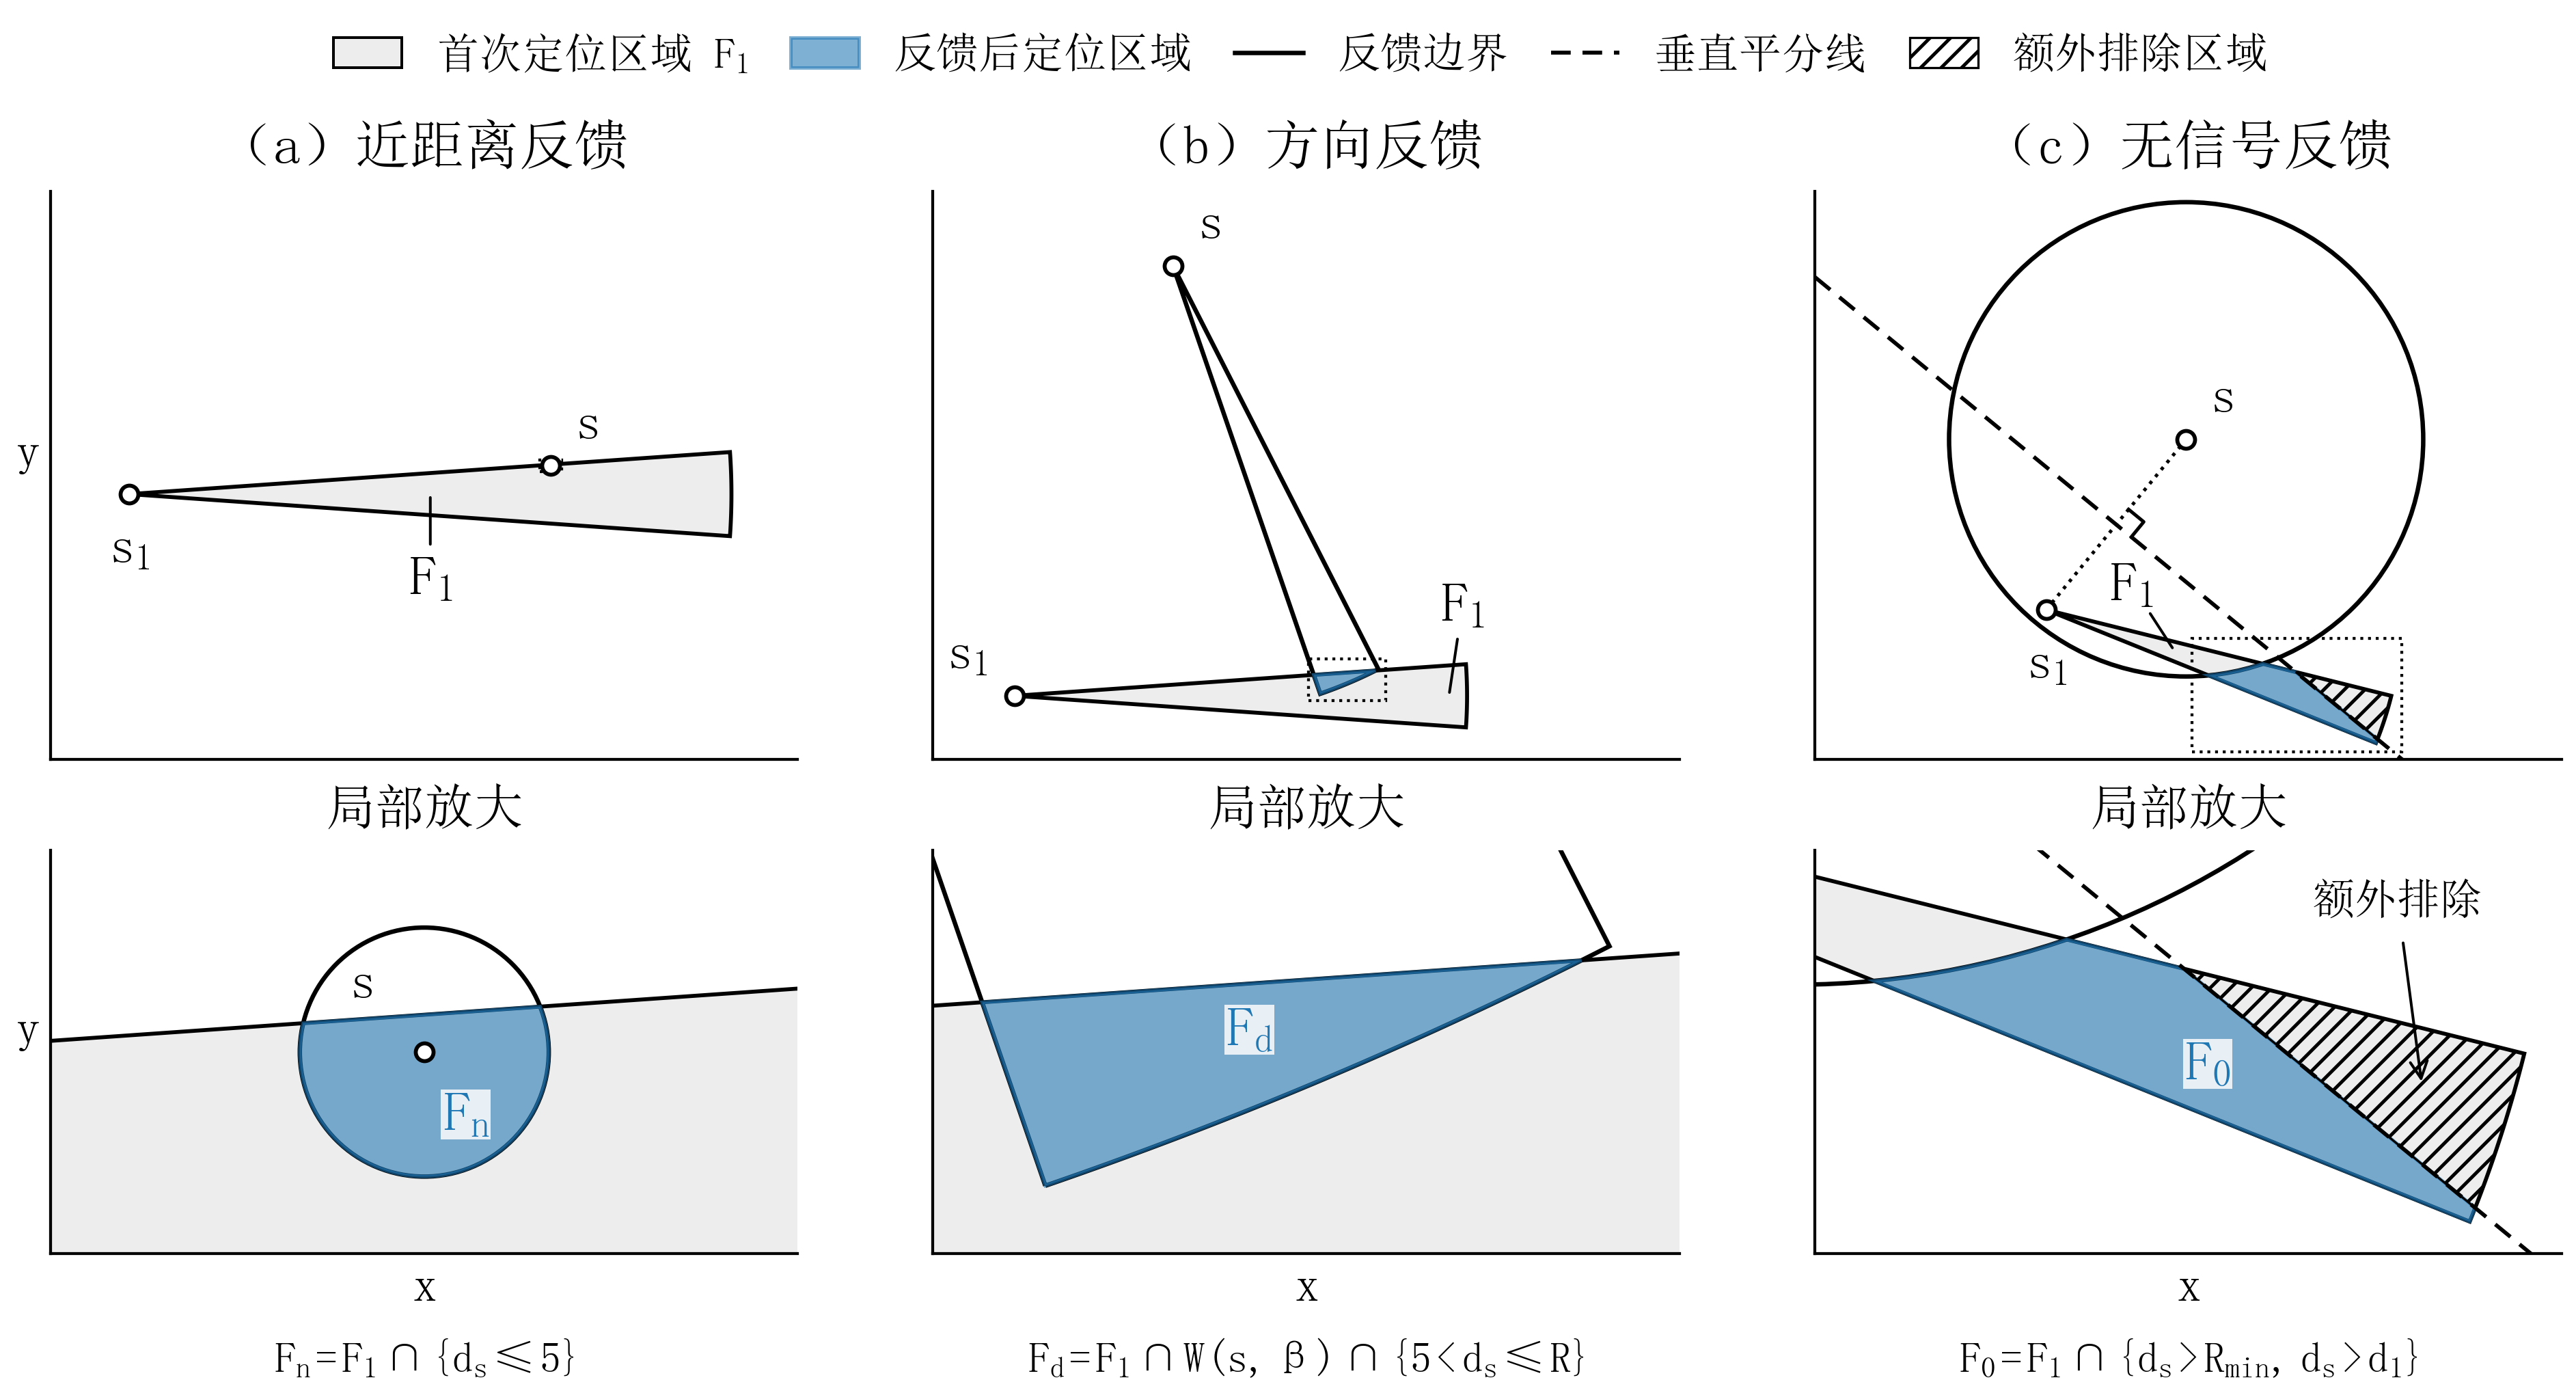
\includegraphics[width=0.96\linewidth,height=0.68\textheight,keepaspectratio]{figures/q2_three_feedback_schematic.png}
\caption{三类反馈下的定位区域更新}\label{fig:old3}
\end{figure}

\subsection{最小包围圆半径与定位损失}

\subsubsection{定位效果指标的选定}

纯方位观测中的几何布局会影响可观测性与定位精度\textsuperscript{\cite{ref3,ref5}}。本问在反馈之后交付干扰源预测位置，由于干扰源位置一定在定位区域内，故评价标准是预测位置到定位区域内点的最大距离。评价指标须同时给出预测位置的几何中心与误差上界，但问题一所用的区域直径 \(D(P)\) 只刻画角度交会区域的跨度，而本问所需的两项指标由最小包围圆一并给出，所以我们据此替换评价指标。

对非空有界的定位区域 \(F\)，我们选取最坏误差最小的点作为预测位置，以该最小最坏误差作为误差上界：
\[
\hat g(F)\in\arg\min_{c\in\mathbb R^2}\sup_{g\in F}\|g-c\|_2
\,,\qquad
\rho(F)=\min_{c\in\mathbb R^2}\sup_{g\in F}\|g-c\|_2
\tag{15}
\]

其中，\(\hat g(F)\) 为反馈后的预测位置，\(\rho(F)\) 为定位区域 \(F\) 的最小包围圆半径。式（15）表明，\(\hat g(F)\) 为全部预测点中最优的一个，\(\rho(F)\) 为该位置在全部相容位置上的最坏误差，即本次定位在最优预测下达到的误差上界。

该指标的优势在于：可区分直径相同而形状不同的定位区域；与题干第三问20米的光学精确定位距离直接对应：半径不超过20米时，圆心即可作为进入光学作业范围的预测位置。

\subsubsection{最坏定位误差}

由式（15），\(\hat g(F_2(s,y))\) 给出反馈 \(y\) 后的预测位置，\(\rho(F_2(s,y))\) 给出该预测在全部相容位置上的最坏误差。

对于给定的第二检测点 \(s\) 和实际反馈 \(y\)，我们定义单次反馈下的定位损失 \(L(s,y)\) 为该反馈下更新区域能够达到的最小最坏预测误差：
\[
L(s,y)=\rho\bigl(F_2(s,y)\bigr)
\tag{16}
\]

考虑到选择第二检测点时实际反馈尚未发生，此时反馈的可能范围为 \(y\in\mathcal Y(s)\)。我们对检测点 \(s\) 的全部可能反馈取最坏值，定义``最坏反馈定位损失''：
\[
J(s)=\sup_{y\in\mathcal Y(s)}L(s,y)
=\sup_{y\in\mathcal Y(s)}\rho\bigl(F_2(s,y)\bigr)
\tag{17}
\]

为显式展示三类反馈在式（17）中的作用，记检测点 \(s\) 处所有可能返回的方向读数为 \(\mathcal B(s)=\{\beta\in[0^\circ,360^\circ):F_d(s,\beta)\ne\varnothing\}\)，则式（17）等价于：
\[
J(s)=\sup\Bigl(\{\rho(F_d(s,\beta)):\beta\in\mathcal B(s)\}\cup\{\rho(F_k(s)):k\in\{n,0\},\ F_k(s)\ne\varnothing\}\Bigr)
\]

其中，\(k\in\{n,0\}\) 分别对应近距离与无信号反馈。

\(J(s)\) 越小，剩余位置集合在每一种相容反馈下都能由越小的圆覆盖，该检测点的最坏定位效果越好。

\subsection{第二检测点的候选区域与选点策略}

\subsubsection{第二检测点的候选区域}

第二检测点在平面上取任意位置；距离首次定位区域过远的检测点只产生可预先确定的无信号反馈，不提供新的定位信息。记点到集合的距离为：
\[
\operatorname{dist}(s,A)=\inf_{g\in A}\|s-g\|_2,
\]

我们将第二检测点的候选区域确定为：
\[
\mathcal S=
\{s:\operatorname{dist}(s,\overline{F_1})\le1500\}
\tag{18}
\]

对 \(s\notin\mathcal S\) 与任意 \(g\in F_1\) 均有 \(d_s(g)>1500\)，同时有效接收半径满足 \(R\le1500\)，故此时第二次检测必然无信号。故 \(\mathcal S\) 包含全部可能产生信息增益的检测位置，把无限平面上的选点问题限制在此有限候选区域内。

\subsubsection{基于最坏定位误差的第二检测点选址模型}

由式（17），每个检测点 \(s\in\mathcal S\) 对应最坏反馈定位损失为 \(J(s)\)。记搜索域内的最优损失为 \(J^*\)，我们定义``最优二次检测点''：
\[
J^*=\min_{s\in\mathcal S}J(s),\qquad s^*\in\arg\min_{s\in\mathcal S}J(s)
\tag{19}
\]

该检测点具有``最坏情形最优''的数学特点：在所有候选位置中，它使最不利反馈对应的定位损失达到最小。以反馈后定位区域的最小包围圆圆心预测时，任一相容反馈下的预测误差均不超过 \(J^*\)，且其他检测位置无法提供更小的统一误差上界，因此该点具有针对反馈不确定性的最优误差保障。

\subsection{最优二次检测点的求解}

上述模型包含位置搜索、方向反馈枚举及曲边区域求交。我们采用``粗网格与局部增密搜索算法''，对各候选点统一计算三类反馈后的最小包围圆半径，并据此提取近优候选集。

\textbf{Step 1　构造首次定位区域。} 输入第一次检测位置 \(s_1\)、示向度 \(\theta_1\) 及题设常量，按式（9）构造首次定位区域 \(F_1\)，并保留位置与有效接收半径之间的对应关系。若 \(F_1=\varnothing\)，则判定观测结果不相容。

\textbf{Step 2　离散第二检测点候选区域。} 式（18）给出的候选区域为连续集合，无法逐点计算，因此先以100米为间距生成位置网格，并将网格点作为第二检测点的有限候选。

\textbf{Step 3　计算最坏定位损失。} 对每个候选位置 \(s\)，构造三类反馈对应的定位区域并计算其最小包围圆半径，取所有可能反馈下的最大半径作为该位置的最坏定位损失 \(\widehat J(s)\)。

\textbf{Step 4　逐级增密位置网格迭代最优位置。} 比较各网格点的 \(\widehat J(s)\)，在损失较小的区域依次将网格间距缩小为20米、2米和0.5米，并重复Step 3，得到更精确的第二检测位置。

以首次检测点为原点、示向度为\(0^\circ\)为例，数值搜索结果如图\ref{fig:q2-station-search}所示，算法伪代码见附录B。

\begin{figure}[H]
\centering
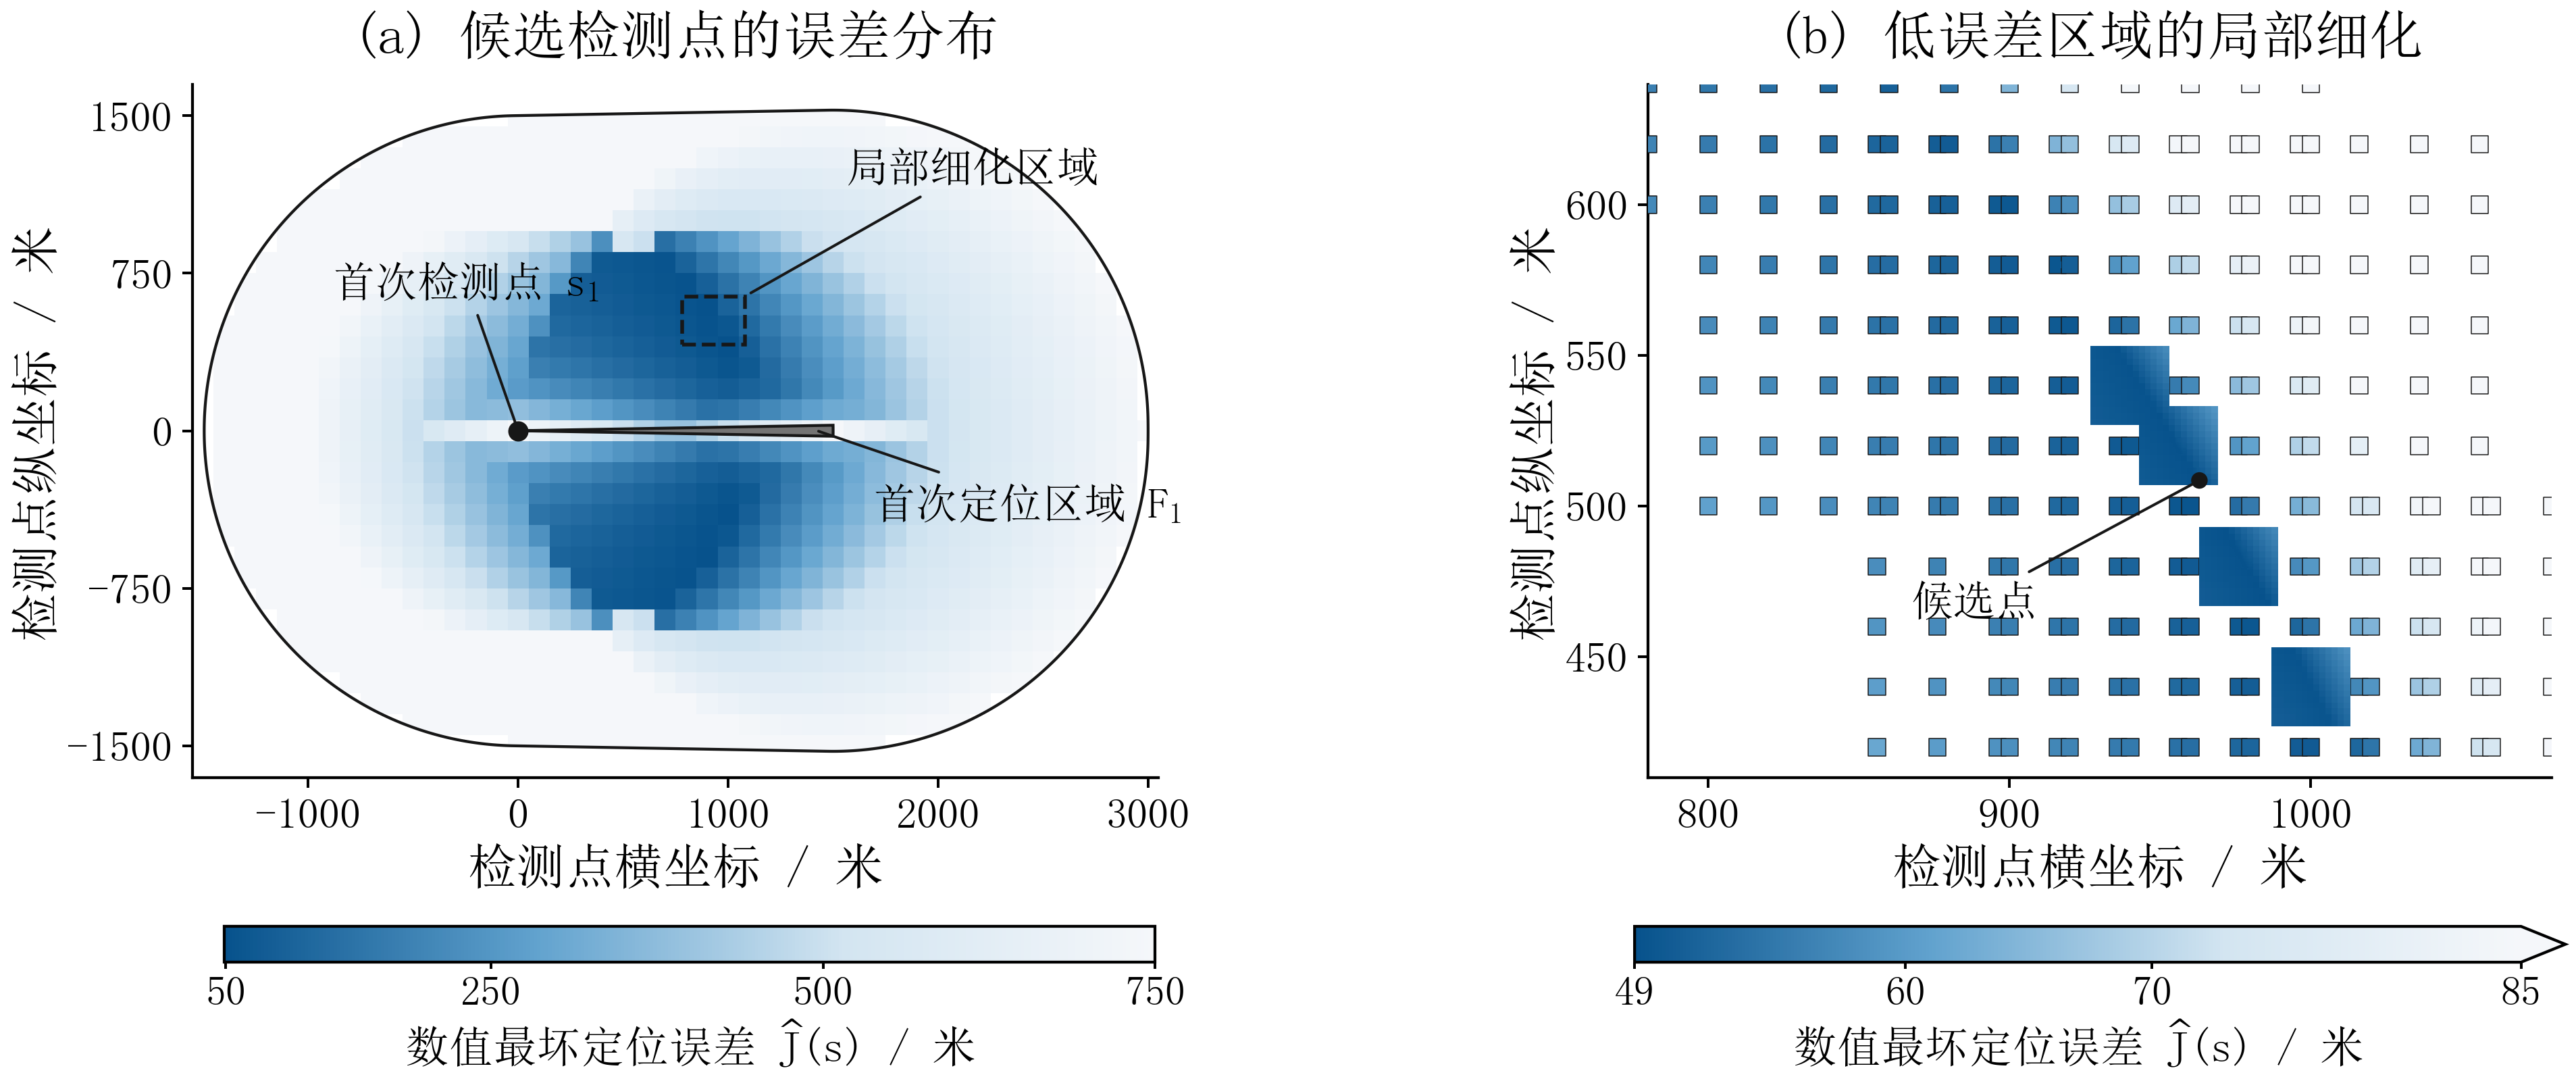
\includegraphics[width=\linewidth]{figures/q2_station_search.png}
\caption{候选检测点的最坏定位误差分布与局部细化}\label{fig:q2-station-search}
\end{figure}

\subsection{预测精度与选点作用检验}

我们以预测位置与真实位置的距离为依据，开展配对模拟实验，分别检验新增观测与检测点选择对定位精度的影响。

\subsubsection{测试设置与评价指标}

按演练生成规则构造模拟场景，源中心在目标圆域内留有30米边界余量，其余参数按演练分布抽样，测向误差采用按频道区分的固定平滑误差场。选取首次在原点获得方向反馈的5000例，三条规则在相同场景与首次观测下开展配对测试。

记规则 \(\pi\) 的预测位置为 \(\hat g_\pi\)、首次反馈为 \(Y_1\)，定义条件均方误差及均方根误差：
\[
\mathcal R(\pi;s_1)
=\mathbb E\!\left[
\|\hat g_\pi-g\|_2^2
\mid Y_1=\text{方向},s_1
\right],
\qquad
\mathcal E(\pi;s_1)=\sqrt{\mathcal R(\pi;s_1)}
\]

对 \(N=5000\) 个样本，令 \(e_i=\|\hat g_i-g_i\|_2\)，以样本均方根误差评价整体定位精度：
\[
\widehat{\mathcal E}
=\sqrt{\frac1N\sum_{i=1}^{N}e_i^2}
\]

该指标以米为单位，数值越小，整体定位精度越高。

\subsubsection{选点规则与预测结果}

我们设置表\ref{tab:old4}所示的三条规则。比较``仅用首次观测''与``随机选取第二点''，检验新增观测的作用；比较两条二次检测规则，检验相同观测次数下的选点优化效果。

\begingroup
\small
\setlength{\tabcolsep}{4pt}
\setlength{\TableInnerWidth}{\dimexpr\linewidth-4\tabcolsep\relax}
\renewcommand{\arraystretch}{1.22}
\begin{longtable}{@{}>{\centering\arraybackslash}p{0.250\TableInnerWidth}>{\centering\arraybackslash}p{0.120\TableInnerWidth}>{\centering\arraybackslash}p{0.630\TableInnerWidth}@{}}
\caption{观测与选点规则}\label{tab:old4}\\
\toprule
规则 & 观测次数 & 第二点选择 \\
\midrule
\endfirsthead
\multicolumn{3}{c}{表\thetable\quad 观测与选点规则（续）}\\
\toprule
规则 & 观测次数 & 第二点选择 \\
\midrule
\endhead
\midrule
\multicolumn{3}{r}{续下页}\\
\endfoot
\bottomrule
\endlastfoot
仅用首次观测 & 1 & 不增加第二次观测 \\
随机选取第二点 & 2 & 在式（18）的搜索外包域内按面积均匀抽样，每例抽取一次 \\
本文选点规则 & 2 & 按首次示向度旋转预先求得的代表点 \\
\end{longtable}
\endgroup

三条规则均采用最小包围圆圆心预测源位置。其中，仅用首次观测时，以 \(\hat g(F_1)\) 作为预测位置；采用两次观测时，两条规则使用相同的反馈更新与位置估计方法。

三条规则在同批5000例上的预测误差如表\ref{tab:old5}所示。

\begingroup
\small
\setlength{\tabcolsep}{4pt}
\setlength{\TableInnerWidth}{\dimexpr\linewidth-8\tabcolsep\relax}
\renewcommand{\arraystretch}{1.22}
\begin{longtable}{@{}>{\centering\arraybackslash}p{0.250\TableInnerWidth}>{\centering\arraybackslash}p{0.190\TableInnerWidth}>{\centering\arraybackslash}p{0.200\TableInnerWidth}>{\centering\arraybackslash}p{0.160\TableInnerWidth}>{\centering\arraybackslash}p{0.200\TableInnerWidth}@{}}
\caption{同批5000例的预测误差}\label{tab:old5}\\
\toprule
规则 & 均方根误差 / 米 & 平均距离误差 / 米 & 中位数 / 米 & 95\%分位数 / 米 \\
\midrule
\endfirsthead
\multicolumn{5}{c}{表\thetable\quad 同批5000例的预测误差（续）}\\
\toprule
规则 & 均方根误差 / 米 & 平均距离误差 / 米 & 中位数 / 米 & 95\%分位数 / 米 \\
\midrule
\endhead
\midrule
\multicolumn{5}{r}{续下页}\\
\endfoot
\bottomrule
\endlastfoot
仅用首次观测 & 333.828 & 281.789 & 263.149 & 610.216 \\
随机选取第二点 & 229.057 & 151.509 & 66.078 & 512.487 \\
本文选点规则 & 12.091 & 10.543 & 9.611 & 21.444 \\
\end{longtable}
\endgroup

由表\ref{tab:old5}，随机增加一次观测使均方根误差由333.828米降至229.057米；在同为两次观测的条件下，本文规则进一步降至12.091米，较随机选点减少216.965米。上述结果表明，在该测试分布下，本文选点规则仅需两次观测即可达到10米级的整体定位精度，体现了检测点优化在有限观测条件下的定位优势。

三条规则的预测误差累积分布如图\ref{fig:q2-error-ecdf}所示，右图进一步放大小误差区间。

\begin{figure}[H]
\centering
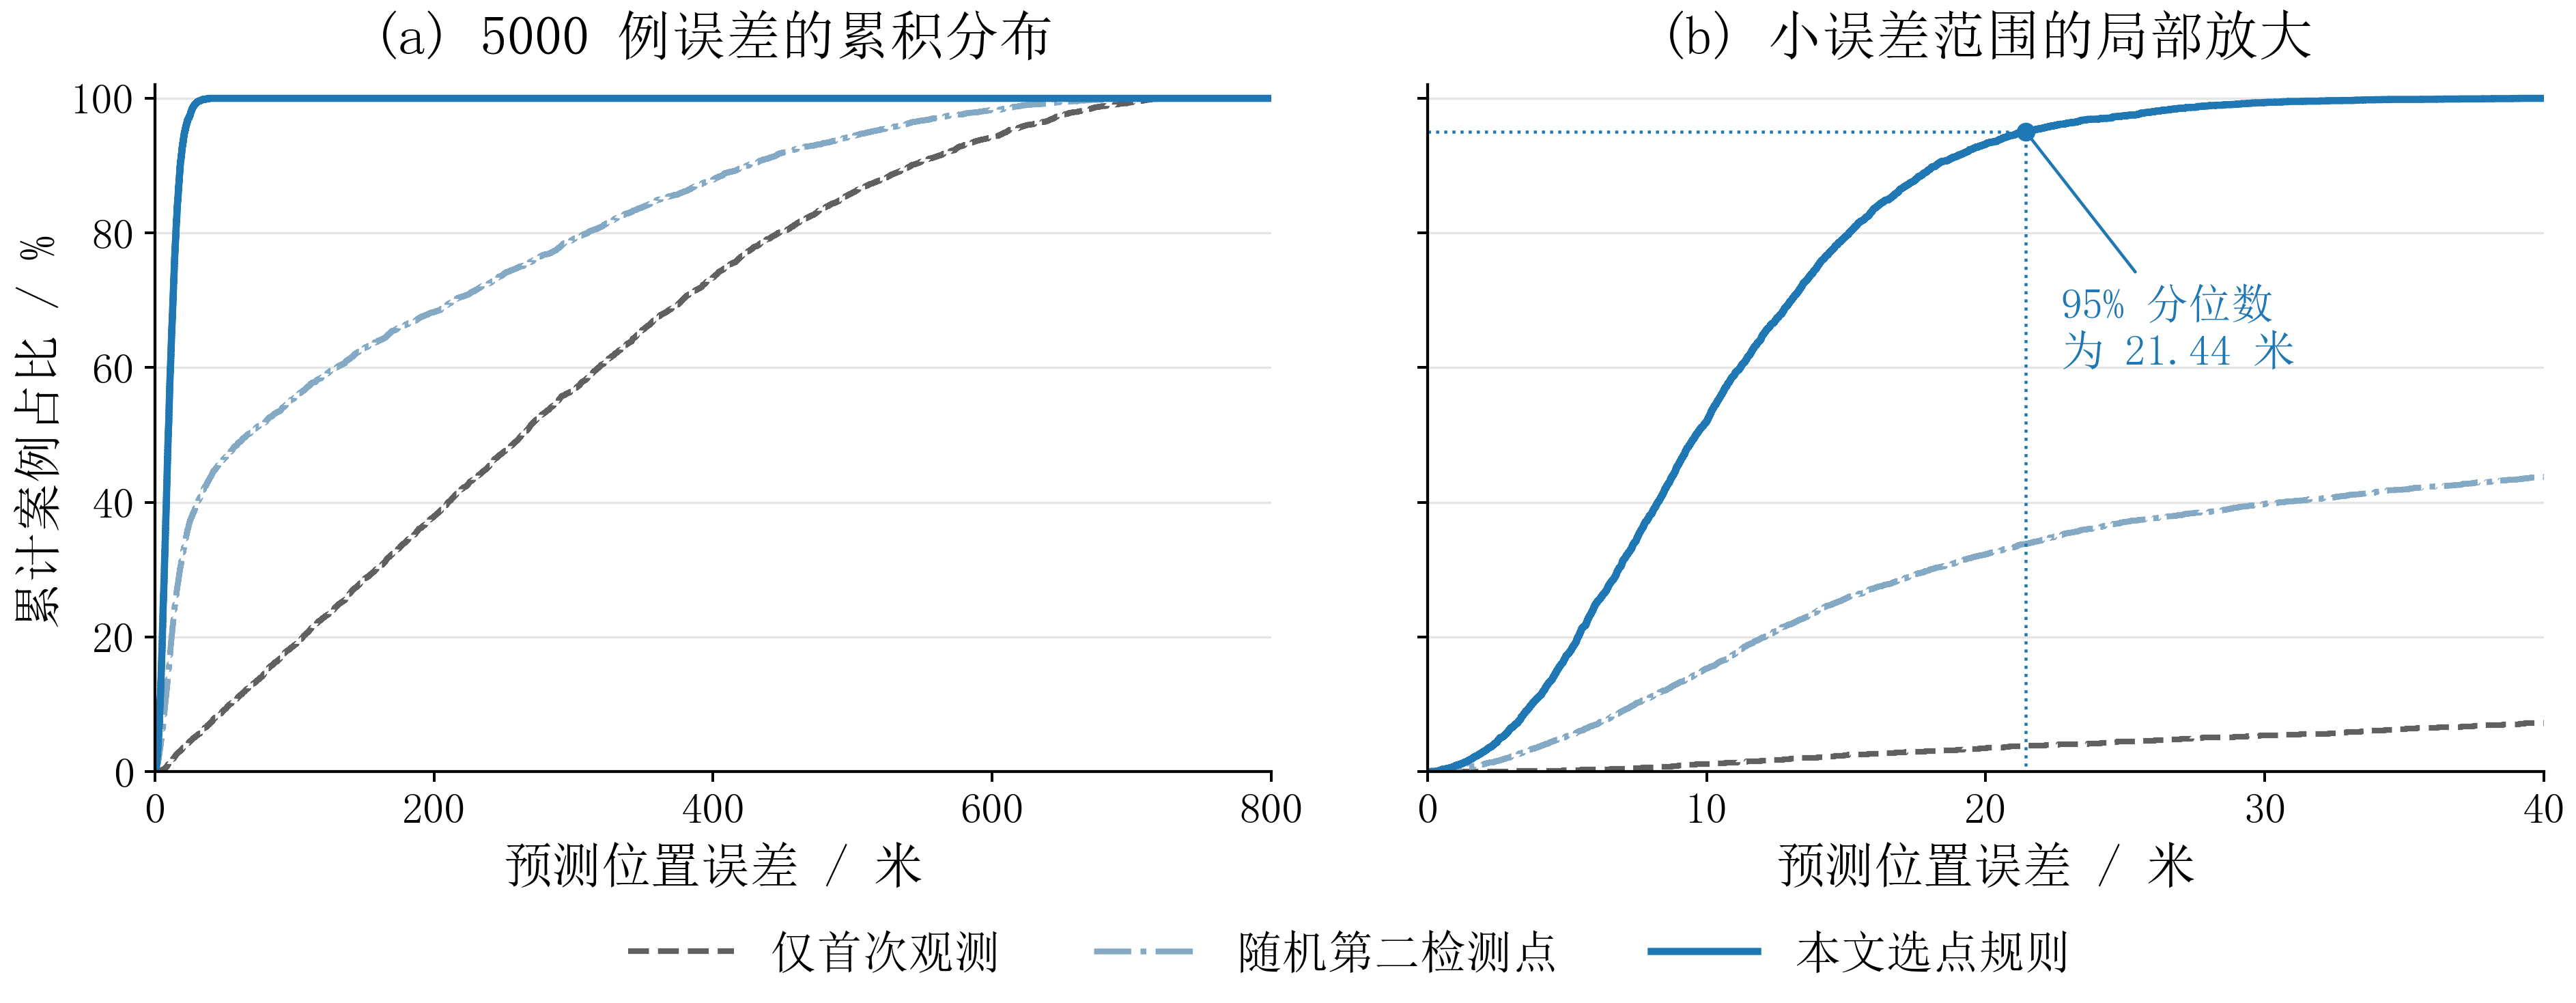
\includegraphics[width=\linewidth]{figures/q2_prediction_error_ecdf.png}
\caption{同批5000例中三种规则的预测误差累积分布}\label{fig:q2-error-ecdf}
\end{figure}
